\renewcommand{\appendixname}{Anexo}
\renewcommand{\thechapter}{\Alph{chapter}}

% Comando para iniciar la sección de anexos en el índice
\newcommand{\initappendix}{%
  \phantomsection%
  \addcontentsline{toc}{chapter}{Anexo}%
}

% Comando para cada anexo individual
\newcommand{\anexo}[1]{%
  \refstepcounter{chapter}%
  \chapter*{Anexo \thechapter: #1}%
  \addcontentsline{toc}{section}{Anexo \thechapter: #1}%
  \markboth{Anexo \thechapter: #1}{}%
}

\clearpage
\initappendix

\anexo{Propuesta de Tema}\label{anexo:propuesta}

\vspace*{\fill}

\noindent A continuación se incluye, de forma completa, la Propuesta de Tema formalmente aprobada por la cátedra al inicio del proyecto (alumno: D'Elia, Matías Nicolás -- tutor: Salas, Joaquín). Se agrega como respaldo documental y administrativo del proyecto. El desarrollo real y sus decisiones técnicas -- incluida la evolución respecto de lo originalmente propuesto -- se documentan en el cuerpo principal de este informe, particularmente en el Capítulo 1 (Marco Teórico, Sección 1.2).

\vspace*{\fill}

\clearpage
\thispagestyle{empty}
{\hoffset=0pt\voffset=0pt
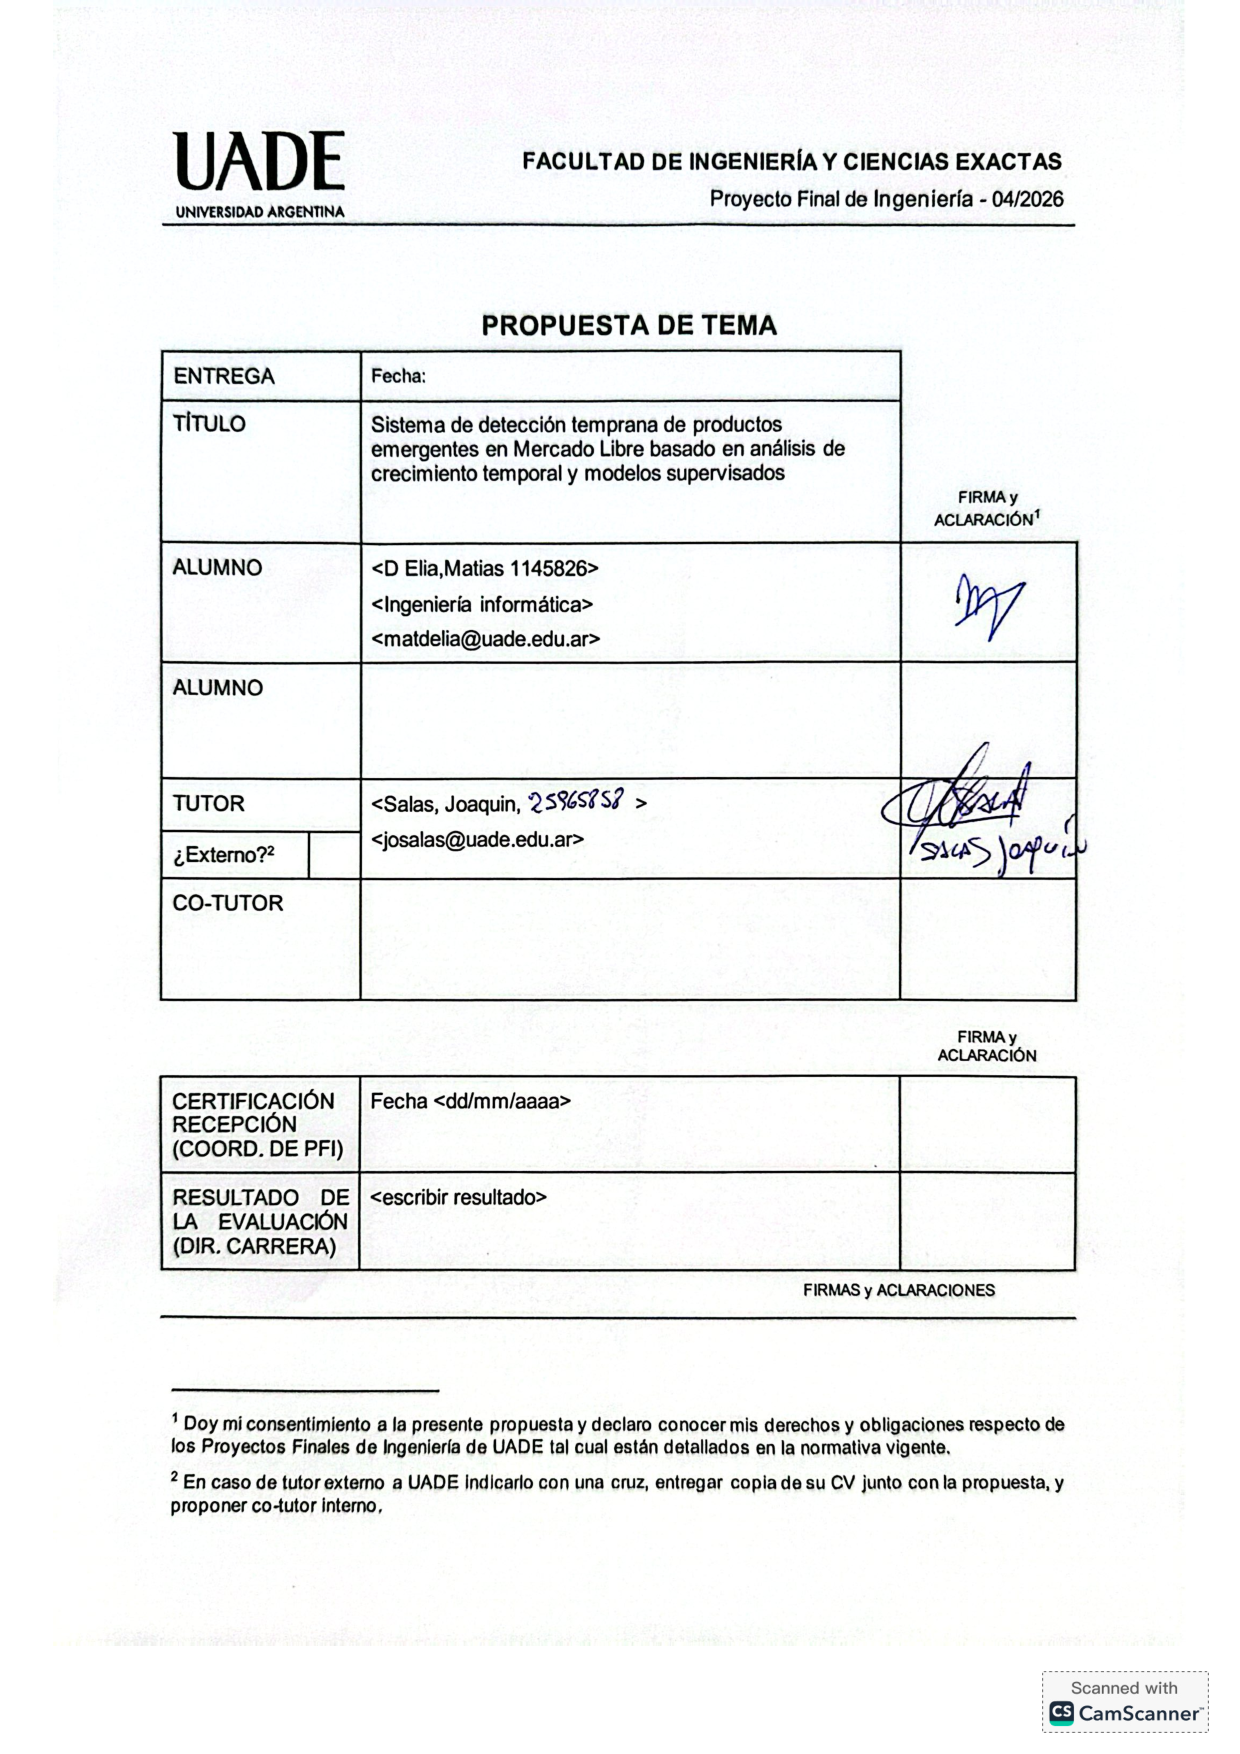
\includepdf[pages=-, pagecommand={\thispagestyle{empty}}]{cover/propuesta_tema.pdf}}
\clearpage
 % Propuesta de Tema aprobada, como respaldo documental/administrativo
\anexo{Cronograma de Actividades}

Las columnas del cronograma representan los cuartos del calendario planificado para todo el PFI (25\,\%, 50\,\%, 75\,\% y 100\,\% del tiempo total del proyecto), y el sombreado indica en qué cuarto se trabajó cada actividad, en base al historial real de desarrollo (commits y bitácoras de sesión). Los cuartos ya transcurridos (25\,\%, 50\,\% y 75\,\%) tienen fecha calendario asociada; el cuarto 100\,\% todavía no tiene fecha de entrega fijada por la cátedra al momento de esta entrega, y se deja indicado como ``a definir'' en lugar de estimarse arbitrariamente. Esta entrega corresponde al hito del 75\,\%: además de las actividades ya en curso desde el cuarto anterior, se sumaron el entrenamiento y evaluación del primer modelo de Machine Learning supervisado, el desarrollo del modelo de negocio, la viabilidad económica y el branding, y (a partir de observaciones puntuales de la revisión oral del hito del 50\,\%) un sistema de cuentas y autenticación, la resolución de la identidad de producto por catálogo, la agregación del score entre vendedores y un endurecimiento de seguridad sobre las cuentas. El análisis final de resultados y la redacción completa del informe (incluyendo Resumen, Abstract y Agradecimientos) corresponden a la última etapa del proyecto y todavía no se iniciaron.

\newcommand{\avance}{\cellcolor{black!75}}

\begin{table}[ht]
	\centering
	\small
	\renewcommand{\arraystretch}{0.85}
	\caption{Cronograma de actividades}
	\label{tab:gantt}
	\begin{tabularx}{\textwidth}{@{}X c c c c@{}}
		\toprule
		\textbf{Actividad} & \textbf{\footnotesize 25\% (Abr--May 26)} & \textbf{\footnotesize 50\% (Jun--Ago 26)} & \textbf{\footnotesize 75\% (Sep 26)} & \textbf{\footnotesize 100\% (a definir)} \\
		\midrule
		Definición del problema y alcance                    & \avance &         &         &         \\
		Marco teórico y antecedentes académicos               & \avance & \avance &         &         \\
		Estado del arte y comparación de herramientas          & \avance & \avance &         &         \\
		User Research y validación inicial                    & \avance & \avance &         &         \\
		Definición de arquitectura general                    & \avance & \avance &         &         \\
		Diseño del modelo de datos en PostgreSQL               & \avance & \avance &         &         \\
		Conexión con API oficial de Mercado Libre              & \avance & \avance &         &         \\
		Construcción del pipeline de captura de datos          & \avance & \avance &         &         \\
		Construcción del dataset histórico propio              & \avance & \avance & \avance &         \\
		Desarrollo del backend con Next.js (API Routes)        & \avance & \avance &         &         \\
		Implementación del motor analítico                    &         & \avance &         &         \\
		Desarrollo del dashboard web                          & \avance & \avance &         &         \\
		Cálculo de métricas temporales                        &         & \avance &         &         \\
		Entrenamiento y evaluación del modelo de ML supervisado &         &         & \avance &         \\
		Modelo de negocio, viabilidad económica y branding     &         &         & \avance &         \\
		Sistema de cuentas, autenticación y alertas            &         &         & \avance &         \\
		Identidad de producto por catálogo y score agregado    &         &         & \avance &         \\
		Endurecimiento de seguridad (rate limiting, cambio de contraseña) &  &        & \avance &         \\
		Pruebas funcionales y ajustes                         & \avance & \avance & \avance &         \\
		Análisis de resultados y limitaciones                 &         &         & \avance &         \\
		Redacción final y preparación de defensa               &         &         &         &         \\
		\bottomrule
	\end{tabularx}
\end{table} % En las entregas que no son la entrega final, se debe tener al menos un anexo con el cronograma (Gantt)
\anexo{Resultados de la Encuesta}

Se presentan a continuación los gráficos de resultados generados automáticamente por Google Forms, correspondientes a la encuesta de 120 respuestas descripta en el capítulo de User Research (sección de Objetivo de la encuesta, Composición de la muestra y Resultados por segmento).

\begin{figure}[ht]
	\centering
	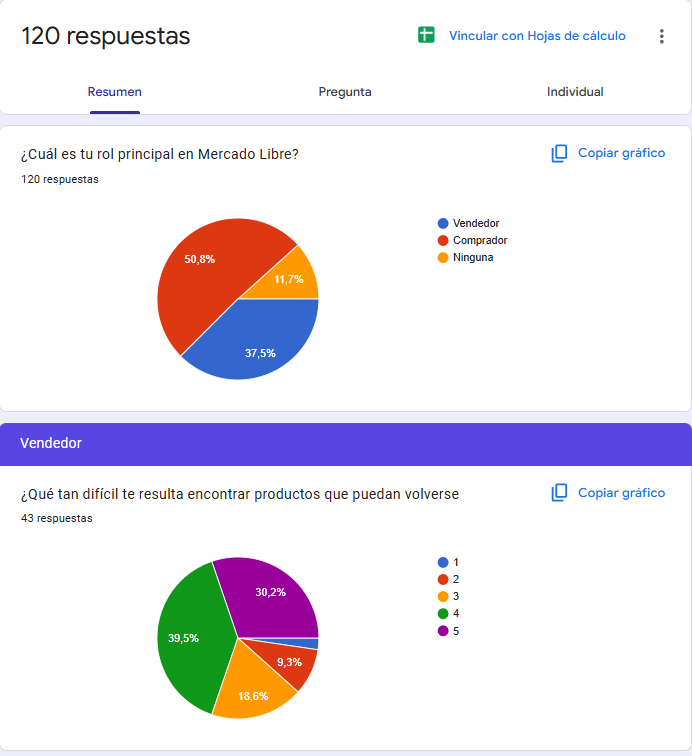
\includegraphics[width=0.68\textwidth]{./images/encuesta/encuesta1Tesis.png}
	\caption{Resultados de la encuesta en Google Forms (120 respuestas, cierre 16/07/2026): rol principal y dificultad para encontrar productos en tendencia.}
	\label{fig:encuesta-1}
\end{figure}

\begin{figure}[ht]
	\centering
	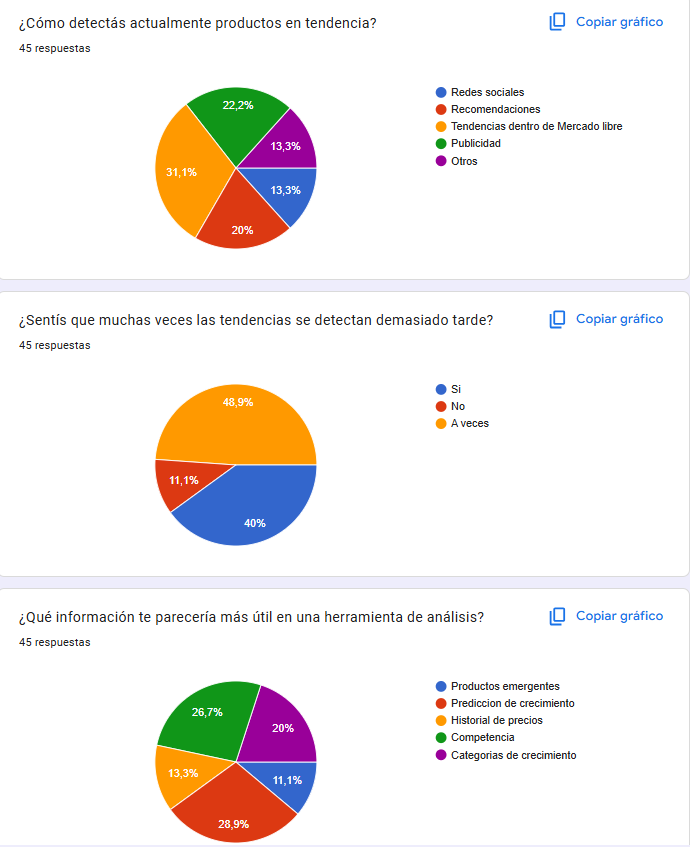
\includegraphics[width=0.68\textwidth]{./images/encuesta/encuesta2Tesis.png}
	\caption{Resultados de la encuesta en Google Forms: método de detección, percepción de detección tardía e información más útil.}
	\label{fig:encuesta-2}
\end{figure}

\begin{figure}[ht]
	\centering
	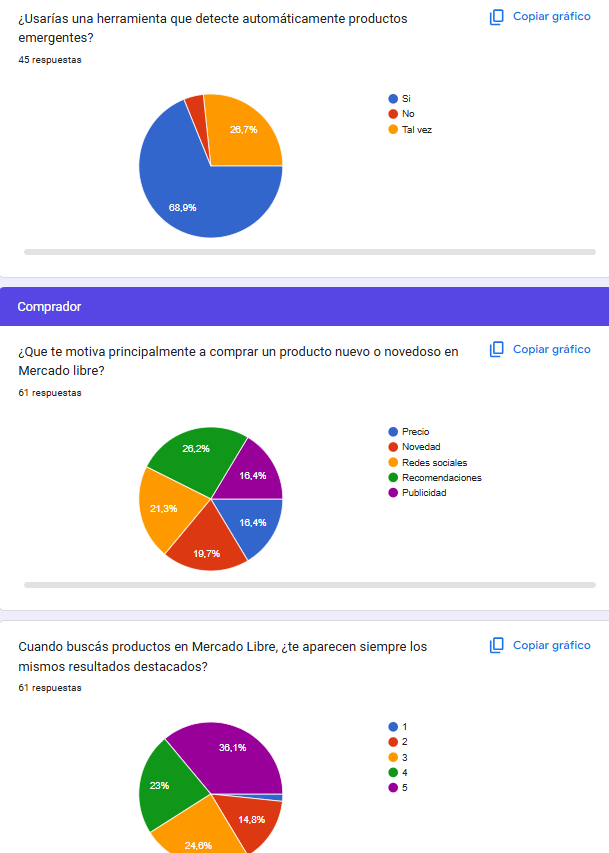
\includegraphics[width=0.68\textwidth]{./images/encuesta/encuesta3Tesis.png}
	\caption{Resultados de la encuesta en Google Forms: disposición a usar una herramienta automatizada y motivación de compra.}
	\label{fig:encuesta-3}
\end{figure}

\begin{figure}[ht]
	\centering
	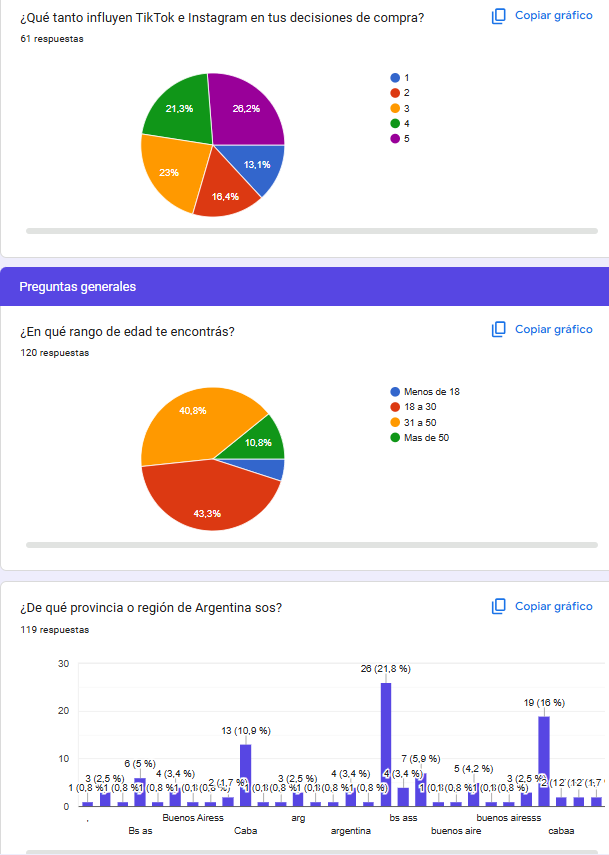
\includegraphics[width=0.68\textwidth]{./images/encuesta/encuesta4Tesis.png}
	\caption{Resultados de la encuesta en Google Forms: influencia de redes sociales, rango de edad y distribución geográfica.}
	\label{fig:encuesta-4}
\end{figure} % En el caso de tener en cuestas tiene que haber una transcripción de los resultados
\anexo{Entrevista 1: Vendedor de Mercado Libre (foco: la problemática)}

Como complemento cualitativo de la encuesta, se realizaron tres entrevistas semiestructuradas a usuarios reales de Mercado Libre: dos vendedores y una compradora, seleccionados por muestreo intencional entre personas con actividad verificable en la plataforma (no se buscan perfiles profesionales ni expertos, sino usuarios comunes, en línea con el público objetivo de la herramienta). El propósito es profundizar en el porqué de los patrones cuantitativos observados en la encuesta: la detección tardía de tendencias (88,9\% combinado), la alta disposición a usar una herramienta automatizada (68,9\%) y el peso de las señales sociales en la decisión de compra (47,5\%). Cada entrevista se registró con consentimiento informado y se analiza mediante síntesis temática en la Capítulo~\ref{chapter06} (User Research). Los nombres utilizados en las tres transcripciones (este anexo y los Anexos E y F) son pseudónimos elegidos para preservar el anonimato de los entrevistados (Sección~\ref{sec:viabilidad-legal}); no se registran apellidos, datos de contacto ni otra información identificatoria. A continuación se presenta el resumen completo de la primera entrevista, pregunta por pregunta, reportando en tercera persona lo que respondió el entrevistado.

\emph{Entrevistado}: Martín, 34 años. Vende en Mercado Libre hace 4 años, rubro bazar y hogar / gadgets ``virales''.

\emph{Objetivo}: entender el proceso real de decisión de stock y dimensionar el costo de detectar tendencias tarde.

\begin{enumerate}
	\item \textbf{¿Hace cuánto vendés en Mercado Libre, en qué rubro y qué tan seguido incorporás productos nuevos?} Contó que vende hace 4 años en el rubro bazar y hogar, principalmente gadgets de cocina y productos que se vuelven virales (freidoras, organizadores, luces). Suma productos nuevos una o dos veces por mes, cuando algo se repite mucho en redes sociales.
	\item \textbf{Contame la última vez que sumaste un producto nuevo: ¿cómo decidiste que convenía?} Relató que la última incorporación fue una organizadora de placard que vio explotar en TikTok: la vio en más de diez videos distintos en una semana, buscó en Mercado Libre qué oferta había, notó que había pocos vendedores y que vendían poco (menos de 100 unidades), pidió precio a su importador y calculó el margen con envío. Aclaró que no usó ningún sistema para decidir, sino intuición combinada con lo que veía en redes.
	\item \textbf{¿Qué fuentes usás hoy para saber qué se está vendiendo o qué está creciendo?} Mencionó TikTok e Instagram (reels de ``cosas de hogar''), Google Trends, los ``Buscados'' de Mercado Libre, seguir a cuatro o cinco vendedores grandes para ver qué publican, y un grupo de WhatsApp de vendedores donde se intercambian tips. Señaló que Mercado Libre Analytics solo le sirve para ver su propia venta, no la del mercado en general, y que eso es justamente lo que le falta.
	\item \textbf{¿Cuánto tiempo por semana le dedicás a investigar tendencias o productos para stockear?} Estimó unas 3 o 4 horas por semana, pero las considera mal invertidas: scrollea redes, mira rankings y compara precios a mano, sin llegar a una respuesta clara al final del proceso.
	\item \textbf{¿Te pasó de llegar tarde a una tendencia? Contame el caso y qué consecuencia tuvo.} Sí: contó el caso de las luces proyector de estrellas (galaxy light). Las vio en TikTok en marzo, dudó una semana y pidió muestras; para cuando tuvo stock disponible, ya había 200 publicaciones y el precio de referencia había bajado un 30\%. Compró 40 unidades, vendió 12 a buen precio y liquidó el resto casi a costo. Reconoció que perdió plata y que quedó con miedo de meterse en la siguiente tendencia, un miedo que también tuvo costo, porque a las últimas dos tendencias que vio directamente no entró.
	\item \textbf{Si esa información la hubieras tenido dos semanas antes, ¿qué habrías hecho distinto?} Respondió que habría comprado el doble de stock al precio viejo, publicado antes de que la categoría se saturara y cobrado entre 2 y 3 veces más por unidad, además de arrancar posicionado mientras la demanda todavía estaba creciendo y no cuando ya había 200 competidores. Estimó la diferencia de rentabilidad en una relación de 3 a 1.
	\item \textbf{¿Cómo distinguís una moda pasajera de una tendencia que se va a sostener?} Explicó que mira tres cosas: si la tendencia aparece en cuentas grandes y no solo en cuentas chicas, si se sostiene más de 3 o 4 semanas en redes y en Google Trends (y no es solo un pico de un día), y si en el marketplace todavía hay pocos vendedores pero la búsqueda ya viene creciendo. Dijo que desconfía cuando solo encuentra videos de cuentas chicas con ``link en bio''.
	\item \textbf{¿Qué información te falta hoy y no encontrás en ningún lado?} Señaló que le falta poder ver la velocidad a la que crece la demanda antes de que se note en las ventas: según su experiencia, no existe ningún lugar que indique que un producto está acelerando en tiempo real. Mercado Libre muestra rankings, pero sin velocidad ni historial ni precios históricos, y las ventas de la competencia que se muestran son una estimación que decide la plataforma, no un dato real verificable.
	\item \textbf{¿Probaste alguna herramienta o método para esto (planillas, apps, seguir cuentas)? ¿Qué te aportó?} Contó que probó planillas propias con datos de Google Trends, pero las abandonó a las dos semanas porque daban mucho trabajo; también probó seguir cuentas, el ranking de Mercado Libre y el grupo de WhatsApp de vendedores. De todo eso, lo que más le aportó fue el grupo de WhatsApp, porque hay gente que ya probó cosas y comparte qué funciona y qué no. Consideró que TikTok le sirve para descubrir productos, pero le hace perder mucho tiempo.
	\item \textbf{¿Qué tendría que tener una herramienta para que la uses todas las semanas?} Mencionó tres condiciones: que la herramienta avise sola cuando algo empieza a acelerar (porque si tiene que entrar a revisarla, no la va a usar), que muestre el crecimiento en números simples y estime cuánto puede ganar (margen frente a saturación), y que le insuma menos de 10 minutos por semana. Advirtió que si tuviera que cargar datos manualmente, la abandonaría, como pasó con las planillas.
\end{enumerate}
 % Entrevista 1 (anexo independiente por entrevista: devolucion E50)
\anexo{Entrevista 2: Vendedor de Mercado Libre (foco: validación de la solución)}

Segunda de las tres entrevistas semiestructuradas descriptas en la metodología general del Anexo D. Nombre utilizado es un pseudónimo, en línea con el criterio de anonimización ya explicado (Sección~\ref{sec:viabilidad-legal}).

\emph{Entrevistado}: Lucas, vendedor de Mercado Libre, mostrándole el dashboard del sistema con el ranking y el score de tendencia.

\emph{Objetivo}: validar la comprensión y utilidad del dashboard y del score de tendencia mostrando el sistema en funcionamiento.

\begin{enumerate}
	\item \textbf{¿Qué vendés, hace cuánto, y cómo decidís hoy qué stockear?} Respondió que vende tecnología, y que hoy decide con intuición, combinando redes sociales, el ranking de Mercado Libre y el precio del importador. Lo describió como apostar con datos sueltos.
	\item \textbf{Antes de ver la herramienta: si una aplicación te dijera ``este producto está creciendo'', ¿qué necesitarías saber para creerle?} Indicó que necesitaría saber la fuente del dato (si son ventas reales de Mercado Libre o una estimación), el período de crecimiento, el volumen base (aclaró que pasar de 2 a 10 ventas no es lo mismo que pasar de 500 a 1000) y si el crecimiento es consistente o fue solo un pico de un día. Sin esa información, dijo, el número no significa nada para él.
	\item \textbf{(Mostrando el dashboard) ¿Qué entendés que muestra esta pantalla?} Interpretó que se trata de un ranking de productos ordenados según qué tan en tendencia están, con un puntaje y un desglose de cuánto aparece en búsquedas, hace cuánto viene creciendo, su precio y su posición en el catálogo. En sus palabras, resumió que la pantalla muestra ``lo que está creciendo ahora''.
	\item \textbf{El score va de 0 a 100: ¿qué esperarías de un producto con 80 frente a uno con 40?} Explicó que con un puntaje de 80 esperaría un producto que viene subiendo con fuerza desde hace dos o tres semanas, con volumen real y todavía sin saturar, algo que investigaría el mismo día. Con 40, en cambio, lo consideraría dudoso: podría ser un pico raro o algo recién empezando sin saber si se sostiene, así que lo miraría, pero no arriesgaría stock en base a eso.
	\item \textbf{¿Qué harías mañana con este ranking si fuera tuyo?} Describió que filtraría por su categoría, ordenaría por score y a los tres o cuatro productos mejor rankeados les pediría precio al importador; los que tuvieran poca competencia y buen margen los publicaría esa misma semana, y después configuraría una alerta semanal.
	\item \textbf{De los componentes del score (aparece seguido, se mantiene en el tiempo, posición en el catálogo, precio estable), ¿cuál te importa más? ¿Agregarías alguno?} Dijo que los componentes que más le importan son que se mantenga en el tiempo y la posición en el catálogo, porque aparecer seguido puede ser solo un pico aislado. Como componentes adicionales, propuso sumar la cantidad de vendedores compitiendo (saturación), la velocidad de caída del precio y un margen estimado según el costo típico de la categoría.
	\item \textbf{¿Preferís entrar a mirar el panel o recibir una alerta cuando algo empieza a crecer? ¿Por qué medio?} Prefiere sin dudas la alerta: si tiene que entrar a mirar el panel, lo hace como mucho una vez por semana, y consideró que es justamente la alerta la que evita llegar tarde, que es su problema principal. Sugirió que llegue por WhatsApp o mail, con un mensaje simple del tipo ``este producto está creciendo en tu categoría''.
	\item \textbf{¿Qué le falta a esta herramienta para que la uses en serio en tu operación?} Pidió que el dato sea específico de su categoría y no un ranking genérico de toda la plataforma, que se pueda ver el historial (no solo el score del día) y que se actualice con frecuencia; aclaró que si el dato está desactualizado o es demasiado general, no le sirve para decidir compras de stock.
	\item \textbf{¿La usarías gratis? ¿Pagarías por ella? ¿Qué valor mensual te parecería razonable?} Afirmó que gratis la usaría sin dudarlo, y que también pagaría si de verdad le permitiera entrar dos semanas antes a una tendencia, ya que un solo error de timing en una tendencia le costó más de lo que pagaría en dos años de suscripción. Consideró razonable un rango de entre 10 y 30 dólares mensuales, siempre que la herramienta demuestre que ese costo se recupera en margen.
	\item \textbf{¿Qué es lo que menos te convence de lo que viste?} Lo que menos le convenció fue que el score funcione como una caja negra: si no puede entender por qué un producto tiene 80 puntos, no confía en el dato. También cuestionó que la data de ``apariciones'' no sea la venta real de Mercado Libre, ya que los datos públicos de la plataforma son estimaciones, y pidió que se aclare de dónde sale cada número.
\end{enumerate}
 % Entrevista 2
\anexo{Entrevista 3: Compradora de Mercado Libre}

Tercera de las tres entrevistas semiestructuradas descriptas en la metodología general del Anexo D. Nombre utilizado es un pseudónimo, en línea con el criterio de anonimización ya explicado (Sección~\ref{sec:viabilidad-legal}).

\emph{Entrevistada}: Lucía, 27 años. Compra en Mercado Libre 1--2 veces por semana.

\emph{Objetivo}: profundizar el hallazgo de la encuesta sobre señales sociales (47,5\%) y la percepción de repetición de resultados destacados (59,1\%).

\begin{enumerate}
	\item \textbf{¿Qué tan seguido comprás en Mercado Libre y qué tipo de productos?} Contó que compra bastante seguido, una o dos veces por semana, principalmente artículos de decoración, gadgets, cosas para la casa y regalos, muchas veces por impulso al ver algo en redes sociales.
	\item \textbf{Contame tu última compra de algo nuevo o novedoso: ¿cómo llegaste a ese producto?} Relató que su última compra novedosa fue un organizador de cables que vio en un video de TikTok: el video le mostró el producto, lo buscó en Mercado Libre y compró la publicación con más ventas y reseñas con fotos. Resumió que llegó al producto por el video, pero eligió al vendedor por las reseñas.
	\item \textbf{Cuando algo te lo recomiendan o lo ves en redes (TikTok/Instagram), ¿cuánto influye en que lo termines comprando?} Estimó que 8 de cada 10 compras de productos nuevos las vio antes en redes sociales, pero aclaró que el video solo le genera el deseo inicial: la confianza se la dan las reseñas y las fotos de otros compradores, y que las redes sociales sin reseñas no alcanzan para que compre.
	\item \textbf{¿Confiás más en una recomendación de conocidos, en las reseñas, o en lo que la plataforma te muestra primero?} Ordenó su confianza así: primero las recomendaciones de conocidos, después las reseñas con fotos y videos, y en último lugar lo que la plataforma muestra primero: esto último, dijo, casi no le genera confianza y a veces incluso le provoca rechazo porque lo percibe como publicidad.
	\item \textbf{Cuando buscás algo, ¿sentís que te aparecen siempre los mismos productos destacados? ¿Eso te ayuda o te molesta?} Confirmó que sí, que le aparecen siempre los mismos productos con ``Envíos Full'' y la etiqueta ``Mejor vendido'', incluso filtrando por precio o novedad. Reconoció que a veces eso le ayuda por rapidez, pero también le molesta, porque siente que no ve todas las opciones y que el resultado destacado no siempre es el mejor ni el más barato.
	\item \textbf{¿Alguna vez compraste algo ``que estaba de moda'' y te arrepentiste? ¿Qué señales no viste a tiempo?} Sí: mencionó el caso de unas luces LED de moda que se veían muy bien en el video, pero resultaron de mala calidad, se rompieron a los dos meses y el vendedor ya no existía. En retrospectiva, identificó las señales que no vio a tiempo: pocas reseñas y todas recientes (algo típico de un producto con reseñas infladas), fotos robadas de internet y un precio demasiado bajo comparado con el resto del mercado.
	\item \textbf{¿Comparás precios entre vendedores o vas al primero que aparece? ¿Cómo lo hacés?} Dijo que compara precios entre vendedores salvo que sea una urgencia: ordena por precio más envío, mira ventas y reputación, y elige entre los dos o tres primeros resultados. Para compras baratas (menos de 10 dólares) no le dedica tiempo a comparar y va directo al primero con buena reputación.
	\item \textbf{¿Qué te daría más confianza para descubrir productos nuevos (historial de precios, ver si viene creciendo, opiniones)?} Señaló que lo que más confianza le daría es el historial de precios, para saber si un descuento como ``40\% OFF'' es real o está calculado sobre un precio inflado. También valoraría ver que el producto viene creciendo en ventas y desde cuándo, junto con reseñas reales con fotos; con esa información se animaría a comprarle a vendedores que no conoce.
	\item \textbf{Si pudieras ver que un producto ``viene subiendo hace dos semanas'' o que su precio está estable, ¿cambiaría tu decisión?} Afirmó que sí cambiaría su decisión: que un producto ``viene subiendo hace dos semanas'' le indica que no es una publicación fantasma ni una estafa de un día, sino que otros ya lo compraron y lo validaron. Agregó que un precio estable la tranquiliza, porque le indica que no le están cobrando de más por la moda del momento.
	\item \textbf{¿Qué es lo que más te frustra hoy al comprar algo nuevo en la plataforma?} Mencionó la publicidad camuflada que se repite, la incertidumbre sobre si el precio que ve es justo, y el miedo a las reseñas falsas o a que el producto se rompa. Resumió que comprar algo nuevo es una lotería, porque nunca se sabe si se va a recibir lo que se vio en el video.
\end{enumerate}
 % Entrevista 3